%My header and style options
\documentclass[a4paper, 12 pt, titlepage]{article}
\usepackage[slovene]{babel}
\usepackage[utf8]{inputenc}
\usepackage[T1]{fontenc}

%\usepackage{vicent}
%\usepackage[0T1]{fontenc}

%custom colour package
\usepackage[usenames, dvipsnames]{xcolor}

%graphics, captions etc.
\usepackage[pdftex]{graphicx}
\usepackage{caption}
\usepackage{amssymb, float, amsmath, stackrel, fullpage, slashed, subcaption}

%to get the colourful hyperlinks ... not just square boxes around them ...
\usepackage{hyperref}
\hypersetup{
	colorlinks=true,
	linkcolor=black!60!red,
	citecolor=black!60!green,
	urlcolor=black!60!cyan,
	filecolor=black!60!magenta
}

%set up custom captions
\captionsetup{
	font=small,
	margin=10pt,
	labelfont=it,
	labelsep=endash,
	format=hang,
	width=0.7\textwidth
}

%bibliography
%\usepackage[round]{natbib}

%LOOKS WAY BETTER WITHOUT THESE ... :P
%costum matter fonts and section fonts
%\usepackage{mathpazo}
%\usepackage{sectsty}
%\allsectionsfont{\LARGE\sffamily\bfseries}

\newcommand{\parc}[2]{
	\ensuremath{\frac{\partial#1}{\partial#2}}
}

\newcommand{\vac}[1][\phi]{
	\ensuremath{\langle#1\rangle}
}

%\renewcommand{\to}{
%	\ensuremath{\longrightarrow}
%}

% New definition of square root:
% it renames \sqrt as \oldsqrt
\let\oldsqrt\sqrt
% it defines the new \sqrt in terms of the old one
\def\sqrt{\mathpalette\DHLhksqrt}
\def\DHLhksqrt#1#2{%
\setbox0=\hbox{$#1\oldsqrt{#2\,}$}\dimen0=\ht0
\advance\dimen0-0.2\ht0
\setbox2=\hbox{\vrule height\ht0 depth -\dimen0}%
{\box0\lower0.4pt\box2}}

\newenvironment{myfig}[2][10cm]
{
	\vspace{-20pt}
	\begin{figure}[H]
		\begin{center}
			\includegraphics[keepaspectratio=1, width=#1]{#2}
		\end{center}
		\vspace{-24pt}
}
{
	\end{figure}
	\vspace{-6pt}
}

\renewenvironment{abstract}[1][1.0]
{
	\begin{center}
		{\bf Abstract}\\[12pt]
		\begin{minipage}{#1\textwidth}
}
{
		\end{minipage}
	\end{center}
}

\begin{document}

%titlepage
\begin{titlepage}
	\begin{figure}[H]
		\centering
		
\includegraphics[width = 7cm, keepaspectratio=1]{pics/logo.pdf}\\[12pt]
		{\sc Oddelek za fiziko}\\[4cm]
	\end{figure}
	\begin{center}
		\large{Seminar -- 2. letnik 2. bolonjske stopnje}\\[0.5cm]
		\LARGE\textbf{Masivna elektrodinamika}\\[1.0cm]

		\vspace{0.0cm}

		\begin{minipage}{0.4\textwidth}\small
			\begin{flushleft}
				\textsc{Author:}\\[0.2cm]
				Jože Zobec
			\end{flushleft}
		\end{minipage}
		\begin{minipage}{0.4\textwidth}\small
			\begin{flushright}
				\textsc{Mentor:}\\[0.2cm]
				Prof. Dr. Borut Bajc
			\end{flushright}
		\end{minipage}
	\end{center}

	\vspace{5.0cm}

	\begin{abstract}
		% try to write something nice for the abstract ;)
	\end{abstract}
	
	\vfill

	\centering{\footnotesize Ljubljana, \today}
\end{titlepage}

%table of contents, obviously ...
\tableofcontents

\pagebreak

%Now the fun stuff begins ...
\section{Introduction}
Higgs boson, the holy grail of particle physics\ldots It has come a long way from just a hypothesis, a
mathematical trick to make the theory more feasible. There are now indications, that it is no joke.

We live perhaps in a unique time, where the discovery of ``Higgs'' might become a reality.
Journalists went so far as to dub it `the God particle'. While such nicknames are nothing but exaggerations, the
discovery of the Higgs boson, will mean that for the last 50 years we've been mostly on the right track, it
will be the so called `experimentum crucis', that will round up and complete the Standard model experimentally
as well.

The theory of particle physics has advanced to such an extent, that many are wondering if this still makes any
sense at all and the 
problem is, that some theories have begun to border on metaphysics, rather than physics\footnote{String theory is such an example.}.
New theories and models have been proposed and we don't know which to follow.

Despite what many theorists would like to think, physics is an empirical science, we study nature. And so theory of nature must be
in agreement with nature itself. If it doesn't describe it, it's not physics anymore.

So in truth it doesn't really matter if we confirm the Higgs boson or reject it (although it would be really
appreciated if we did), because either way it will give us hints and clues on how to continue our description
of nature.


%the more qualitative alternative for Higgs
\section{Ponovitev}

Iz predavanj Vi\v sje kvantne mehanike se spomnimo, da lahko polja
kvantiziramo prek operatorjev polja, za kar pa nujno potrebujemo kreacijske, $a^\dagger$ in 
anihilacijske $a$ operatorje. Na kratko ponovimo nekaj pojmov, s katerimi se bomo sre\v cevali tekom tega
seminarja.

\subsection{Grupa}

\vspace{0.5 cm}

{\em Grupa} je mno\v zica elementov z naslednjimi lastnostmi:

\begin{enumerate}
	\item{Med elementi obstaja asociativna operacija.}
	\item{Mno\v zica je za to operacijo zaprta.}
	\item{Izmed teh elementov je natanko eden tak, ki je za to operacijo enota.}
	\item{V mno\v zici so zajeti tudi vsi inverzni elementi.}
\end{enumerate}

V kolikor ne veljajo vsi pogoji imamo enega izmed ni\v zjih objektov, kot je na primer monoid (nimamo
nujno vseh inverzov) ali polgrupa (nimamo nujno udentitete).

\v Ce je operacija komutativna, je ta grupa abelova in operacijo imenujemo se\v stevanje. Sicer
pa je grupa neabelova in operacijo imenujemo mno\v zenje.

\subsection{Algebra}

\vspace{0.5cm}

Pogostokrat sre\v camo pojem `algebra'. Pa ponovimo, kaj je to.\\

\emph{Kolobar} je mno\v zica elementov z naslednjimi lastnostmi:

\begin{enumerate}
	\item{Ta mno\v zica je abelova grupa z operacijo se\v stevanja.}
	\item{Elementi so hkrati (pol)grupa za operacijo mno\v zenja.}
	\item{Za kombinacijo operacij velja distributivnostna relacija.}
\end{enumerate}

\emph{Algebra} je vektorski prostor nad kolobarjem.

Liejeve grupe imajo tudi svojo algebro -- generatorji Liejevih grup nepenjajo vektorski
prostor na mnogoterosti grupe\footnote{Vsaka Liejeva grupa je hkrati mnogoterost}. Da poka\v zemo,
da zado\v s\v cajo pogojem iz algebre zado\v s\v ca zapis komutacijskih relacij med generatorji, zato
bomo na tem mestu definirali komutator, en.~\eqref{komutator} in anti-komutator, en.~\eqref{antikomutator}:

\begin{align}
	[A,B] &\equiv AB - BA, \label{komutator}\\
	\{A,B\} &\equiv AB + BA. \label{antikomutator}
\end{align}

Vpeljali bomo skupno notacijo, s katero bomo lahko "`me\v sali"' med obema pojmoma:

\begin{align}
	[A,B]_\pm = AB \pm BA.
\end{align}

Tudi kon\v cnim grupam lahko priredimo algebre -- za nas relevantna je simetri\v cna grupa
$S_n$, ki jo imenujemo tudi permutacijska grupa.

\v Ce to grupo raz\v sirimo z operacijo parnosti, ima ta nova grupa dve nerazcepni upodobitvi. Funkcije so lahko
bodisi simetri\v cne na permutacije, ali pa anti-simetri\v cne. Baza za prvo upodobitev so bozonski, za drugo
pa fermionski kreacijsko-anihilacijski operatorji.

Lastne vrednosti so $\pm 1$ (parnost), hkrati pa grupa komutira s Hamiltonianom, kar pomeni,
da je to dobra simetrija in da Hamiltonian lahko zapi\v semo tako, v bazi te upodobitve, oz. druga\v ce:
Hamiltonian lahko zapi\v semo s pomo\v cjo fermionskih ali bozonskih kreacijsko-anihilaijckih operatorjev.

Tako od tu dobimo fermionsko in bozonsko algebro:

\begin{align}
	[a_i, a_j^\dagger]_\pm &= \delta_{ij}, \\
	[a_i, a_j]_\pm &= 0,
\end{align}

kjer komutatorji ustrezajo bozonom, antikomutatorji pa fermionom.

\section{Uvod v supersimetrijo}

Pa si omo\v cimo noge v vodi supersimetrije: obravnavajmo Schr\" odingerjevo ena\v cbo, tj. Hamiltonian

\begin{equation}
	H = -\frac{\hbar^2}{2m}\nabla^2 + mV(\vec{x}).
	\label{schroedinger}
\end{equation}

Vpeljemo enote $\hbar = c_0 = \varepsilon_0 = 1$. Maso $m$ bomo zaenkrat postavili na $1$. Tako je brezdimenzijska
Schr\" odingerjeva ena\v cba

\begin{equation}
	H = -\frac{1}{2}\nabla^2 + V(\vec{x}),
	\label{s1}
\end{equation}

kjer velja \v se $H = i\pt$. V eni dimenziji se~\eqref{s1} glasi

\begin{equation}
	H = -\frac{1}{2}\px^2 + V(x).
	\label{sx}
\end{equation}

Predpostavimo, da je na\v s potencial neni\v celen in navzdol omejen.

Velja

\begin{equation}
	H\psi_n(x) = E_n\psi_n(x) = i\pt\psi_n(x).
\end{equation}

Za $E_0 = 0$ torej velja $H|\psi_0\rangle = 0$. Od tu dobimo pogoj za potencial

\begin{equation}
	V(x) = \frac{1}{2}\frac{\px^2\psi_0}{\psi_0},
	\label{vpogoj}
\end{equation}

kjer smo predpostavili, da so stanja $\psi_n(x)$ vezana stanja, tj. je $\psi_0(x)$ dobro dolo\v cen, in
to lahko storimo.

Na\v s Hamiltonian bi radi zapisali v obliko z operatorjem \v stetja, $a^\dagger$ in $a$, se pravi
$H = a^\dagger a$, zato moramo poiskati nek pameten razcep. Vidimo, da je~\eqref{sx} oblike
$H \sim (A + B)(A - B)$, tako bomo definirali superpotencial $W(x)$, da bo

\begin{align}
	a &= W(x) + \frac{1}{\sqrt{2}}\px, \\
	a^\dagger &= W(x) - \frac{1}{\sqrt{2}}\px.
\end{align}

Taka operatorja sta res drug drugemu hermitsko adjungirana, saj je operator $\px$ anti-hermitski (do totalnega
odvoda natan\v cno).

Vse lepo in prav, vendar, a tak $W (x)$ sploh obstaja? V fiziki na taka vpra\v sanja ponavadi odgovorimo
retrospektivno in to bomo storili tudi sedaj. Vse skupaj vstavimo v Hamiltonian in iz njega dolo\v cimo
vezi, katerim mora zado\v s\v cati.

Poglejmo, kaj naredi $a^\dagger a$ na neki funkciji $\phi (x)$:

\begin{align}
	a^\dagger a\ \phi(x)&= \Big[W(x) - \frac{1}{\sqrt{2}}\px\Big]\Big[W(x) +
		\frac{1}{\sqrt{2}}\px\Big]\phi(x) \notag \\
	&= \Big[-\frac{1}{2}\px^2 + W^2(x)\Big]\phi(x) - \frac{1}{\sqrt{2}}\Big[
		\underbrace{\px \big(W(x)\phi(x)\big) - W(x)\px\phi(x)}_{(\px W(x))\phi(x)} \Big] \notag \\
	&= \bigg\{-\frac{1}{2}\px^2 +
		\underbrace{W^2(x) - \frac{1}{\sqrt{2}}\big[\px W(x)\big]}_{V(x)}\bigg\}\phi(x),
	\label{dokaz.aad}
\end{align}

Se pravi, \v ce je ta ena\v cba Schr\" odingerjeva, potem mora $W (x)$ spo\v stovati slede\v ca izraza:

\begin{align}
	V(x) &=\frac{1}{2}\frac{\px^2\psi_0(x)}{\psi_0(x)} = W^2(x) - \frac{1}{\sqrt{2}}\px
		W(x) \label{riccati} \\
	W(x) &= -\frac{1}{\sqrt{2}}\frac{\px\psi_0(x)}{\psi_0(x)} \label{superpotencial},
\end{align}

kjer smo izraz~\eqref{superpotencial} dobili z re\v sevanjem Riccatijeve ena\v cbe~\eqref{riccati}.

Tako smo dobili $H_1 = a^\dagger a$ in ima re\v sitve $\psi_n(x)$ in $E_n$, kot jih poznamo
od prej.

Poglejmo, kaj se zgodi, \v ce vrstni red obrnemo. Definirajmo \v se $H_2 = aa^\dagger$. Dobimo ga kot

\begin{align}
	H_1 &= -\frac{1}{2}\px^2 + V_1(x) = a^\dagger a, \\
	H_2 &= -\frac{1}{2}\px^2 + V_2(x) = aa^\dagger,
\end{align}

kjer

\begin{align}
	V_1(x) &= W^2(x) - \frac{1}{\sqrt{2}}\px W(x), \notag \\
	V_2(x) &= W^2(x) + \frac{1}{\sqrt{2}}\px W(x). \label{v2pot}
\end{align}

Ena\v cbo~\eqref{v2pot} lahko doka\v zemo z istim postopkom kot~\eqref{dokaz.aad}, le da na funkcijo $\phi(x)$
delujemo z operatorjem $aa^\dagger$.

$H_1$ ima lastne pare $\psi^{(1)}_n(x)$, $E^{(1)}_n$, $H_2$ pa $\psi^{(2)}_n(x)$, $E^{(2)}_n$.

Pravimo, da je $V_2(x)$ supersimetri\v cni partner $V_1(x)$. Lastne funkcije in energijski spekter $H_2$
dobimo lahko z re\v sevanjem, ali pa uganemo

\begin{equation}
	\psi^{(2)}_n(x) = a\psi^{(1)}_n(x),
\end{equation}

od koder vidimo da $\psi^{(2)}_0(x)$ ne obstaja, saj anihilacijski operator iz vakuuma naredi
ni\v clo po definiciji. Energijski spekter $H_2$ je enak tistemu iz $H_1$, s tem da nima
osnovnega stanja $E_0$, kar lahko poka\v zemo kot

\begin{align}
	H_2\psi^{(2)}_n(x) &= aa^\dagger (a\psi^{(1)}_n(x)) = a(a^\dagger a)\psi^{(1)}_n(x) = \notag \\
		&= aE^{(1)}_n\psi^{(1)}_n(x) = E_n^{(1)}(a\psi_n^{(1)}) = E_n^{(1)}\psi_n^{(2)},
	\label{degenener}
\end{align}

se pravi

\begin{equation}
	E^{(1)}_n \equiv E^{(2)}_n, \qquad n = 1, 2, 3 \ldots
\end{equation}

Zaradi tega, spremenimo definicijo $H_1$ tako, da ne bo imel ve\v c osnovnega stanja
\begin{equation}
	H_1 \to H_1^\prime = H_1 - E_0.
\end{equation}

Funkcije hamiltoniana $H_2$ bi morali v dobiti spet z re\v sevanjem 

Hamiltoniana $H_1$ in $H_2$ bi radi zdru\v zili v enega, tako da se prostora ne me\v sata. Zato
definiramo

\begin{equation}
	\H \equiv H_1 \oplus H_2 \equiv \begin{bmatrix}H_1 & \\
		& H_2 \end{bmatrix},
\end{equation}

\begin{equation}
	Q^\dagger = \sigma^+ a^\dagger = \begin{bmatrix} 0 & a^\dagger \\
		0 & 0 \end{bmatrix}, \quad
	Q = \sigma^- a = \begin{bmatrix} 0 & 0 \\
		a & 0 \end{bmatrix},
\end{equation}

\begin{equation}
	Q^\dagger Q + QQ^\dagger = \{Q, Q^\dagger\} = \H.
\end{equation}

\subsection{Me\v sanje bozonskih in fermionskih stanj}

Kot se verjetno kar najbolj povdarja, obstaja v supersimetri\v cnih teorijah nekak\v sna direktna linija,
ki povezuje bozonske operatorje s fermionskimi. Pa poglejmo, kaj to pravzaprav pomeni. Operatorja
$a$ in $a^\dagger$ tvorita boznonsko algebro

\begin{equation}
	[a, a^\dagger] = (\px W), \qquad [a, a] = 0.
\end{equation}

V splo\v snem je $\px W = 1$ le za harmonski oscilator, za vi\v sje \v clene pa je problem bolj
kompliciran, zarade anharmonske sklopitve. Opis v Fockovem prostoru ni ve\v c tako enostaven, vendar
mi verjemite na besedo, da so to \v se vedno bozonski operatorji.

Definirajmo operatorje $c$ in $c^\dagger$, tako da

\begin{equation}
	c = \sigma^+, \qquad c^\dagger = \sigma^-,
\end{equation}

Poka\v zemo lahko, da tile operatorji zadostijo enostavni fermionski algebri,

\begin{equation}
	\{c, c^\dagger\} = 1, \qquad \{c, c\} = 0,
\end{equation}

torej lahko $Q$ in $Q^\dagger$ zapi\v semo kot

\begin{equation}
	Q = c^\dagger a, \qquad Q^\dagger = a^\dagger c.
\end{equation}

Sedaj vidimo, kako je pravzaprav treba interpretirati operatorje $Q$ in $Q^\dagger$. Ker namre\v c
velja

\begin{equation}
	[Q, H] = [Q^\dagger, H] = 0,
\end{equation}

tile operatorji me\v sajo bozonska in fermionska stanje ne da bi pri tem spremenili energijo stanja.

\subsection{Zlom supersimetrije}

Tak Hamiltonian ima degeneriran spekter, saj imata $H_1$ in $H_2$ iste lastne vrednosti. Kadar velja
$E^{(1)}_0 = 0$ pravimo, da je supersimetrija zlomljena, saj Hamiltoniana nista ve\v c degenerirana
in takih operatorjev $Q$ nimamo ve\v c. V teorijah polja to merimo s tako imenovanim Witten-ovim
indeksom,

\begin{equation}
	\Delta (\beta) = \Tr\big[\e^{-\beta H_1} - \e^{-\beta H_2}\big].
\end{equation}

Za supersimetri\v cne teorije je 
\begin{equation}
	\lim_{\beta \to 0} \Delta(\beta) = 0,
\end{equation}
za teorije z zlomljeno supersimetrijo pa 

\begin{equation}
	\lim_{\beta \to 0} \Delta (\beta) = 1,
\end{equation}

saj osnovno stanje $H_1$ pre\v zivi.



%search strategies at the LHC
\section{Neskon\v cna potencialna jama}

Stvari je la\v zje razumeti na konkretnem zgledu, zato si bomo pogledali supersimetrijo na primeru neskon\v cne
potencialne jame. Gre za\v cetni\v ski potencial, (vstavi sliko), omejen od $0$ do $1$. Lastne fukcije so potem kar

\begin{equation}
	\psi_n^{(1)} (x) = \frac{1}{2}\sin n\pi x, \quad E_n^{(1)} = \frac{(n\pi)^2}{2}
		\quad n = 1,2,\ldots
\end{equation}

\ni stanja za $n = 0$ ni, ker to stanje ustreza situaciji brez delca\footnote{Verjetnost, da se delec nahaja v jami
je natanko 0.}. Osnovni lastni par je torej za $n = 1$, vendar ga bolj kljub temu ozna\v cil z indeksom 0.

\begin{equation}
	\psi_0^{(1)} (x) = \frac{1}{2}\sin\pi x, \quad \frac{2}{\pi^2}E_0^{(1)} = 1 \neq 0.
\end{equation}

\ni Supersimetrija je v tem primeru zlomljena, saj $E_0 \neq 0$, zato moramo za\v cetnemu Hamiltonianu
od\v steti energijo osnovnega stanja.

\begin{equation}
	(\underbrace{H - E_0^{(1)}}_{H_1})\psi_0^{(1)} = (E_0^{(1)} - E_0^{(1)})\psi_0^{(1)} =
		0\cdot\psi_0^{(1)} = 0. \label{translacija}
\end{equation}

\ni Od tod lahko poi\v s\v cemo superpotencial $W(x)$ iz en.~\eqref{superpotencial}

\begin{equation}
	W(x) = -\frac{1}{\sqrt{2}} \frac{\px \sin \pi x}{\sin \pi x} = -\frac{\pi}{\sqrt{2}}\cot \pi x.
\end{equation}

\ni S pomo\v cjo en.~\eqref{v2pot} lahko poi\v s\v cemo supersimetri\v cnega partnerja neskon\v cne potencialne jame

\begin{equation}
	V_2 (x) = \frac{\pi^2}{2}\bigg(\cot^2 \pi x + \frac{1}{\sin^2 \pi x}\bigg)
		= \frac{\pi^2}{2}\bigg(\frac{1}{\sin^2 \pi x} - 1\bigg),
	\label{pot-nes-jama}
\end{equation}

\ni kar o\v citno ni ve\v c neskon\v cna potencialna jama, za katero dobimo $V_1(x) = \pi^2/2$, ki pa se ravno
prikladno od\v steje s konstantno $E_0^{(1)}$ v ena\v cbi~\eqref{translacija}. Potencial $V_2$ je poseben primer
potenciala Rosen Morse I (tj. triginometri\v cna izvedenka).

Sedaj smo dobili oba Hamiltoniana,

\begin{align}
	H_1 &= -\frac{1}{2}\px^2, \notag \\
	H_2 &= -\frac{1}{2}\px^2 - V_2(x),
\end{align}

\ni od koder lahko \v ze sklepamo, kako bo izgledal supersimetri\v cni Hamiltonian $\H$.

Poglejmo \v se kako izgledajo valovne funkcije $\psi_n^{(2)}(x)$. Za to bomo seveda uporabili
operatorje vi\v sanja in ni\v zanja iz en.~\eqref{degenener}.
Vemo, da $H_2$ nima stanja pri $n = 1$, ampak da se \v stetje za\v cne pri $n = 2$, vendar bomo tudi
sedaj pisali indeks 0. Uporabili bomo identiteto

\begin{align}
	\psi_0^{(2)} (x) = a\psi_2^{(1)} &= -\frac{1}{2\sqrt{2}}(\pi \cot \pi x -
		\px)\sin2\pi x \\
	&= \frac{2\pi}{2\sqrt{2}}(\cos^2\pi x - \cos 2\pi x) = \frac{\pi}{\sqrt{2}}\sin^2\pi x.
\end{align}

Splo\v sen izraz za $\psi_n^{(2)}$ je dolg. Zapisal bom raje le \v se za
$\psi_3^{(2)}$, za $n=3$, tj. prvo vzbujeno stanje $H_2$:

\begin{equation}
	\psi_3^{(2)}(x) \propto \sin (\pi x) \sin (2\pi x),
\end{equation}

\ni Operatorja $a$ in $a^\dagger$ seveda po pretvorbi pokvarita normalizacijo, tako da rezultati niso nujno
normirani.


%previous hunts: LEP, Tevatron
\section{Podobni Hamiltoniani}

Prava mo\v c supersimetrije se poka\v ze pri obravnavi re\v sljivih problemov. Izka\v ze se, da
imamo kon\v cen nabor potencialov, za katere poznamo to\v cne re\v sitve, med njimi pa lahko definiramo
preproste transformacije, ki en potencial preoblikuje v drugega.

Najprej poka\v zimo kaj so podobni potenciali. Imejmo potencial $V_1 (x; \pr_1)$ in potencial
$V_2 (x; \pr_2)$, kjer sta $\pr_1$ in $\pr_2$ urejena nabora parametrov v potencialih. \v Ce sta
$V_1$ in $V_2$ podobna, potem veljajo slede\v ci identiteti:

\begin{align}
	V_2 (x; \pr_1) &= V_1 (x; \pr_2) + R (\pr_1), \\
	\pr_2 &= \underline{f} (\pr_1). \label{osnova}
\end{align}

Prek en.~\eqref{osnova} lahko definiramo cel razred potencialov, ki so podobni $V_1$:

parametre dobimo prek kompozituma funkcije $f$,
\begin{align}
	\pr_2 &= \underline{f} (\pr_1), \notag \\
	\pr_3 &= \underline{f} (\pr_2) = (\underline{f} \circ \underline{f}) (\pr_1), \notag \\
	&\ldots \notag \\
	\pr_n &= (\underbrace{\underline{f} \circ \underline{f} \circ \ldots \circ \underline{f}}_{n-1}) (\pr_1),
\end{align}

potenciali pa so potem

\begin{align}
	V_2 (x; \pr_1) &= V_1 (x; \pr_2) + R (\pr_1), \notag \\
	V_3 (x; \pr_1) &= V_2 (x; \pr_2) + R (\pr_2) = V_1 (x; \pr_3) + R (\pr_1) + R (\pr_2), \notag \\
	&\ldots \notag \\
	V_n (x; \pr_1) &= V_1 (x; \pr_n) + \sum_{k = 1}^{n-1} R (\pr_k),
\end{align}

ki je spet o\v citno podoben $V_1 (x)$. Sedaj dobimo razred podobnih Hamiltonianov,

\begin{equation}
	H_n = - \frac{1}{2}\px^2 + V_n (x;\pr_1) = - \frac{1}{2}\px^2+V_1(x;\pr_n)+\sum_{k = 1}^{n-1}R(\pr_k).
\end{equation}

Ti Hamiltoniani imajo degeneriran spekter, z izjemo vakuumov, ki so o\v citno

\begin{equation}
	E^{(n)}_0 = \sum_{k = 1}^{n - 1} R(\pr_k).
\end{equation}

Ker so spektri degenerirani, sledi da so vakuumske energije teh hamiltonianov sovpadajo z energijami vzbujenih
stanj Hamiltonianov z indeksom $m < n$. Seveda gremo lahko do konca nazaj, pridemo do $m = 1$ in $E^{(1)}_0 = 0$
in tako dobimo celoten vezani spekter Hamiltoniana $H_1$:

\begin{equation}
	E_n^{(1)} (\pr_1) = \sum_{k = 1}^n R (\pr_k).
	\label{v2-pogoj}
\end{equation}

Seveda to pomeni, da $V_2$ (in posledi\v cno $\pr_2$) ne sme biti arbitraren, ampak tak, da zadosti pogoju
en.~\eqref{v2-pogoj}, sicer pademo lahko v poljubno vzbujeno stanje. Tak na\v cin iskanja spektra je dosti
enostavnej\v si, vendar moramo za to poznati funkcijo $\underline{f}$. 

\subsection{Operatorji dviganja}

V prej\v snji sekciji sem na koncu zgleda povedal, da z naivnim pristopom z operatorjem dviganja ali
spu\v s\v canje lahko le pretvarjamo med supersimetri\v cnima potencialoma. Sedaj bom pokazal, kako jih
je treba uporabiti, da z njimi dejansko lahko dvignemo oz. spustimo stanje.

Spet imejmo Hamiltonian $H_1$, za katerega velja $E^{(1)}_0 = 0$, ki ima valovno funkcijo
$\psi_0^{(1)} (x; \pr_1)$. Operatorje $a^\dagger$ bi morali dejansko ves \v cas pisati kot $a^\dagger (x; \pr)$,
saj

\[
	a^\dagger \equiv a^\dagger (x; \pr) \equiv W(x; \pr) - \frac{1}{\sqrt{2}}\px,
\]

Hamiltonian $H_1$ ima supersimetri\v cnega partnerja $H_2$, ki ima degeneriran spekter. $H_2$ zato lahko
obravnavamo ko podoben Hamiltonian, vemo, da se razlikuje ravno za vakuumsko stanje.

Vi\v sja vzbujena stanja moramo o\v citno dobiti kot

\begin{equation}
	\psi^{(1)}_n (x; \pr_1) \propto a^\dagger (x;\pr_1)\ a^\dagger (x;\pr_2)\ \ldots\ a^\dagger (x; \pr_n)\
		\psi^{(1)}_0 (x; \pr_{n+1}),
\end{equation}

Odtod sledi pomembna posledica: supersimetri\v cna partnerja $V_1$ in $V_2$ sta si podobna potenciala, kar
pomeni, da je med njima lahko netrivialna podobsnostna transformacija -- konkretno lahko spet za zgled vzamemo
neskon\v cno potencialno jamo in en.~\eqref{pot-nes-jama}.

Ker je neprikladno ra\v cunati poljubno visok $\pr_k$ na zalogo, se po navadi raje uporabi kar

\begin{equation}
	\psi^{(1)}_n (x; \pr_1) = a^\dagger (x; \pr_1)\ \psi_{n-1}^{(1)} (x; \pr_2),
\end{equation}

ki nam sugerira, da je za dviganje in spu\v s\v canje dejansko dovolj poznavanje supersimetri\v cnih
partnerjev.

Sipalnih stanj se ne bom dotikal.

\subsection{Klasifikacija podobnih potencialov}

Posebej prikladno je, \v ce znamo podobne potenciale, ki pripadjo podobnostnim transformacijam iste ba\v ze,
pogrupirati, saj lahko prek tega z zamahom roke naenkrat re\v simo vse probleme klasi\v cne kvantne mehanike,
kar se jih da analiti\v cno re\v siti.

Splo\v sen problem je \v se nere\v sen, saj pravzaprav splo\v sen re\v sljivi potencial \v se ni definiran.
Je pa fitzikom kljub temu uspelo zaenkrat pokazati, da obstajata dve pasmi podobnih potencialov:

\begin{itemize}
	\item{$\pr^\prime = \pr + \underline{q}$ -- potenciali, podobni na translacije,}
	\item{$\pr^\prime = q\pr$ -- potenciali, podobni na skaliranje.}
\end{itemize}


%Current status at the LHC
\section{Izospektralni Hamiltoniani}

Izospektralni Hamiltoniani v nerelativisti\v cni kvantni mehaniki so taki, ki imajo strogo enake energijske
spektre vezanih stanj in enake transmisijske/refleksijske koeficiente sipalnih stanj. Edino, kar se
med njimi razlikuje, so valovne funkcije in posledi\v cno nekateri momenti ($\langle x \rangle$, $\langle
x^2 \rangle$ \ldots).

Ideja je ta: superpotencial $W(x)$, ki povezuje $V^{(1)}$ in $V^{(2)}$ ni enoli\v cen, zato lahko poi\v scemo
dru\v zino superpotencialov $\tilde{W}$, ki povezujejo $\tilde{V}^{(1)}$ in $V^{(2)}$. Tako dobimo dru\v zino
$\{\tilde{V}^{(1)}(x;\lambda_1)\}$, ki imajo vsi istega supersimetri\v cnega partnerja $V^{(2)}$. Da se bomo ognili
nanavadnim koeficientom bomo delali v enotah $\hbar = 2m = 1$, zaradi \v cesar se bomo iznebili raznoraznih
koeficientov $(\sqrt{2})^{\pm 1}$ (pozor, cele potence \v stevila $2$ ostanejo).

Hamiltoniani, oblike

\begin{equation}
	H = \frac{\d^2}{\d x^2} + \tilde{V}^{(1)} (x;\lambda_1),
\end{equation}

\ni so vsi izospektralni glede na parameter $\lambda_1$.

Recimo, da $W(x)$ ni enoli\v cen. Potem poleg $W(x)$ obstaja \v se $\tilde{W}(x)$, ki prav tako ustreza
en.~\eqref{v2pot}. Najpreprostej\v sa ideja bi bila potem

\begin{equation}
	W(x) \to \tilde{W}(x) = W(x) + \phi(x),
\end{equation}

\ni kjer zahtevamo, da $\tilde{W}(x)$ prav tako uboga en.~\eqref{riccati} za $V^{(2)}(x)$, ki se v teh enotah
glasi

\begin{equation}
	V^{(2)} (x) = W^2(x) + \px W(x) = \tilde{W}^2(x) + \px\tilde{W}(x),
\end{equation}

\ni od koder sledi

\begin{align}
	W^2 + \odv W &= W^2 + \odv W + 2W\phi + \odv \phi + \phi^2, \notag \\
	2W(x)\phi(x) + \phi^2(x) &= -\odv \phi (x), \notag \\
	\frac{2W(x)}{\phi(x)} + 1 &= -\frac{1}{\phi^2(x)}\odv\phi(x),\qquad y(x) = 1/\phi(x), \notag \\
	2W(x)y(x) + 1 &= -\odv y(x).
\end{align}

\ni Ko to ena\v cbo re\v simo, dobimo

\begin{equation}
	\phi(x) = \odv \ln \bigg[\int_{-\infty}^x \psi_0^2(u)\d u + \lambda_1\bigg] =
		\odv \ln \big[\mathcal{I}_1(x) + \lambda_1\big],
\end{equation}

\ni kjer je $\psi_0(x)$ spet normirana funkcija izvornega potenciala $V^{(1)} (x)$.

Dru\v zina potencialov $\tilde{V}^{(1)} (x; \lambda_1)$, ki ima partnerski potencial $V^{(2)}(x)$ je torej

\begin{equation}
	\tilde{V}^{(1)} (x;\lambda_1) = V^{(1)}(x) - 2\frac{\d^2}{\d x^2}\ln\big[\mathcal{I}_1(x) + \lambda_1\big].
\end{equation}

\ni Parameter $\lambda_1$ se je notri pri\v stulil kot integralska konstanta in ne more biti \v cisto poljuben, ampak
$\lambda_1 \notin [0,1]$, tj $\lambda_1 \in \mathbb{R}\text{\textbackslash}[-1,0]$ -- v tistem re\v zimu osnovno stanje
$\psi_0 (x; \lambda_1)$, potenciala $\tilde{V}^{(1)}(x; \lambda_1)$, ni mo\v c normirati. Izvorni potencial $V^{(1)}(x)$
dobimo kot limito $\lambda_1 \to \pm \infty$. Sliki~\ref{sl2} in~\ref{sl3} ka\v zeta primer za harmonski oscilator.

\begin{figure}[H]
	\centering
	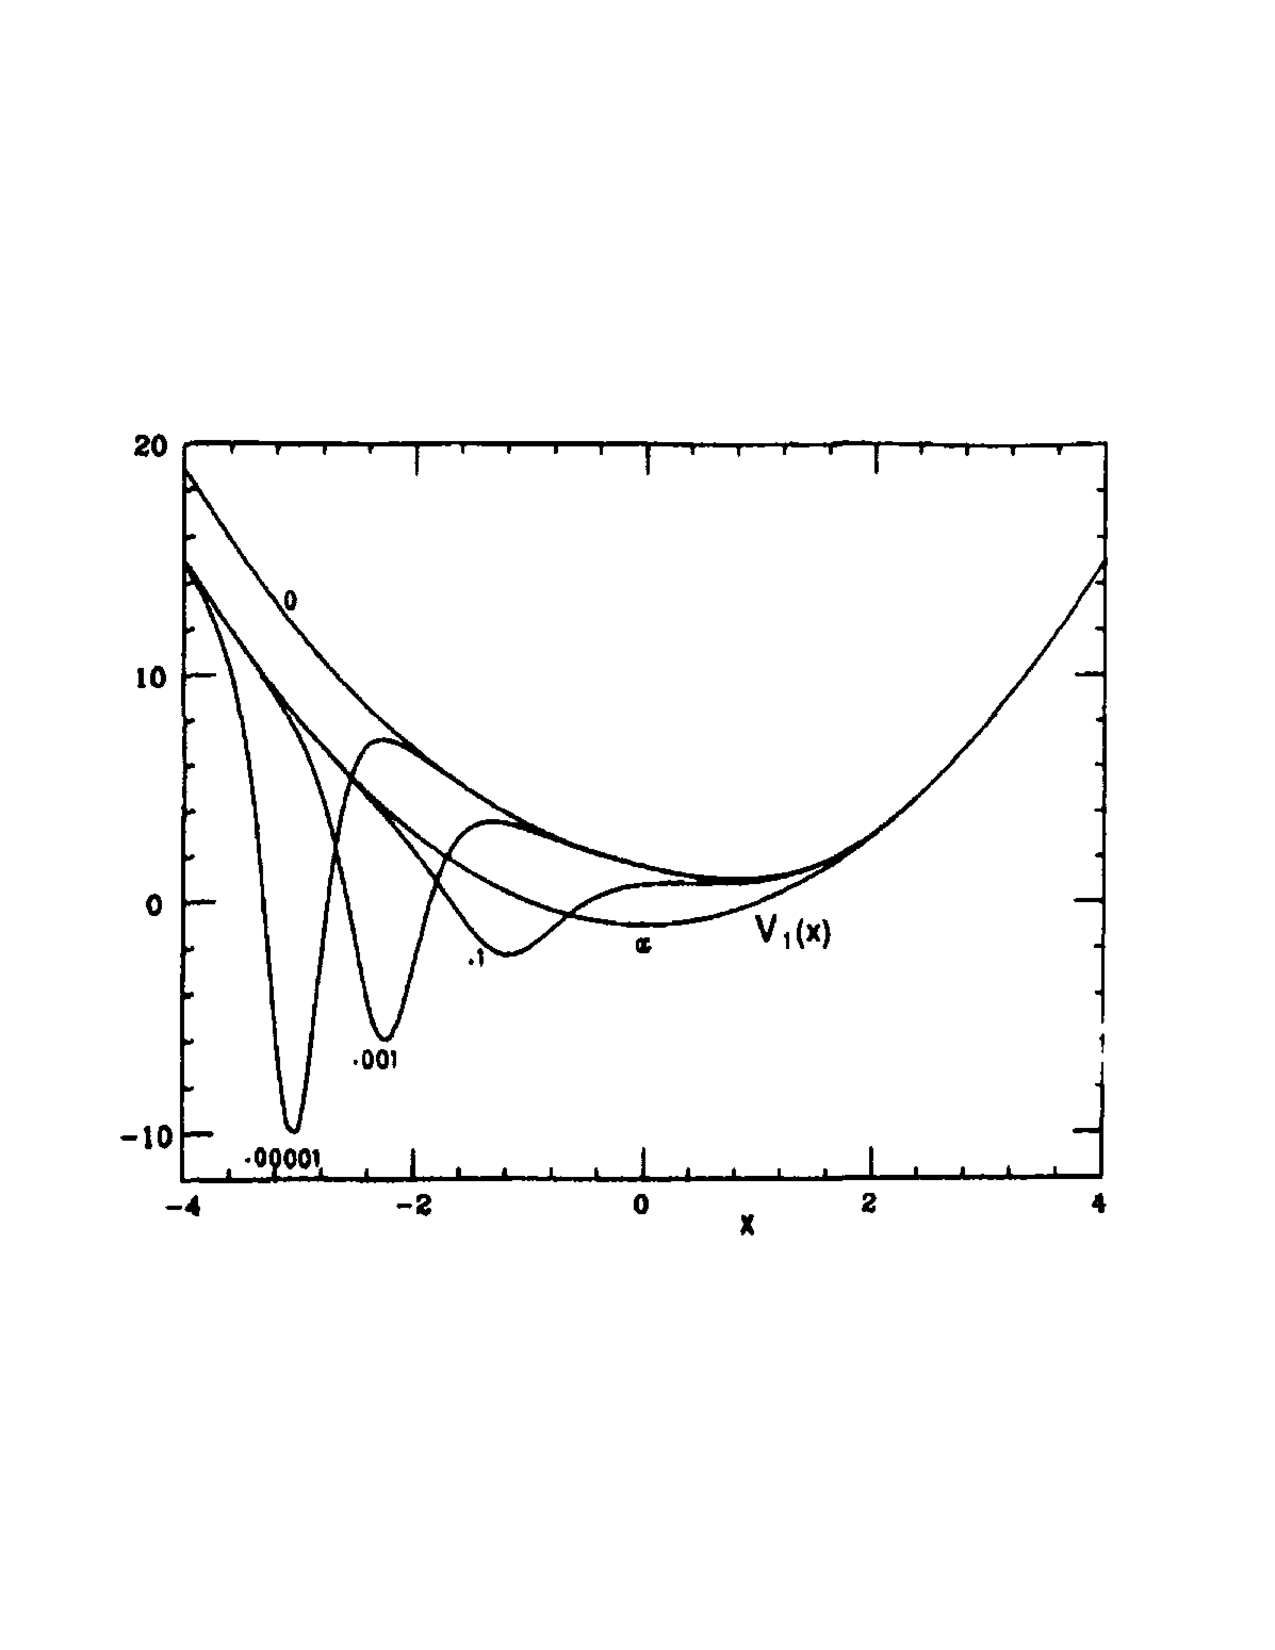
\includegraphics[height=8cm, keepaspectratio=1, trim=0cm 7cm 0cm 7cm]{pics/slika2}
	\caption{Potenciali $\tilde{V}^{(1)}$ za razli\v cne vrednosti $\lambda_1$. Izvorni $V^{(1)}$ je bil Harmonski
		oscilator, ki je tudi prikazan na grafu. Hamiltoniani s temi potenciali so popolnoma izospektralni.}
	\label{sl2}
\end{figure}

\begin{figure}[H]
	\centering
	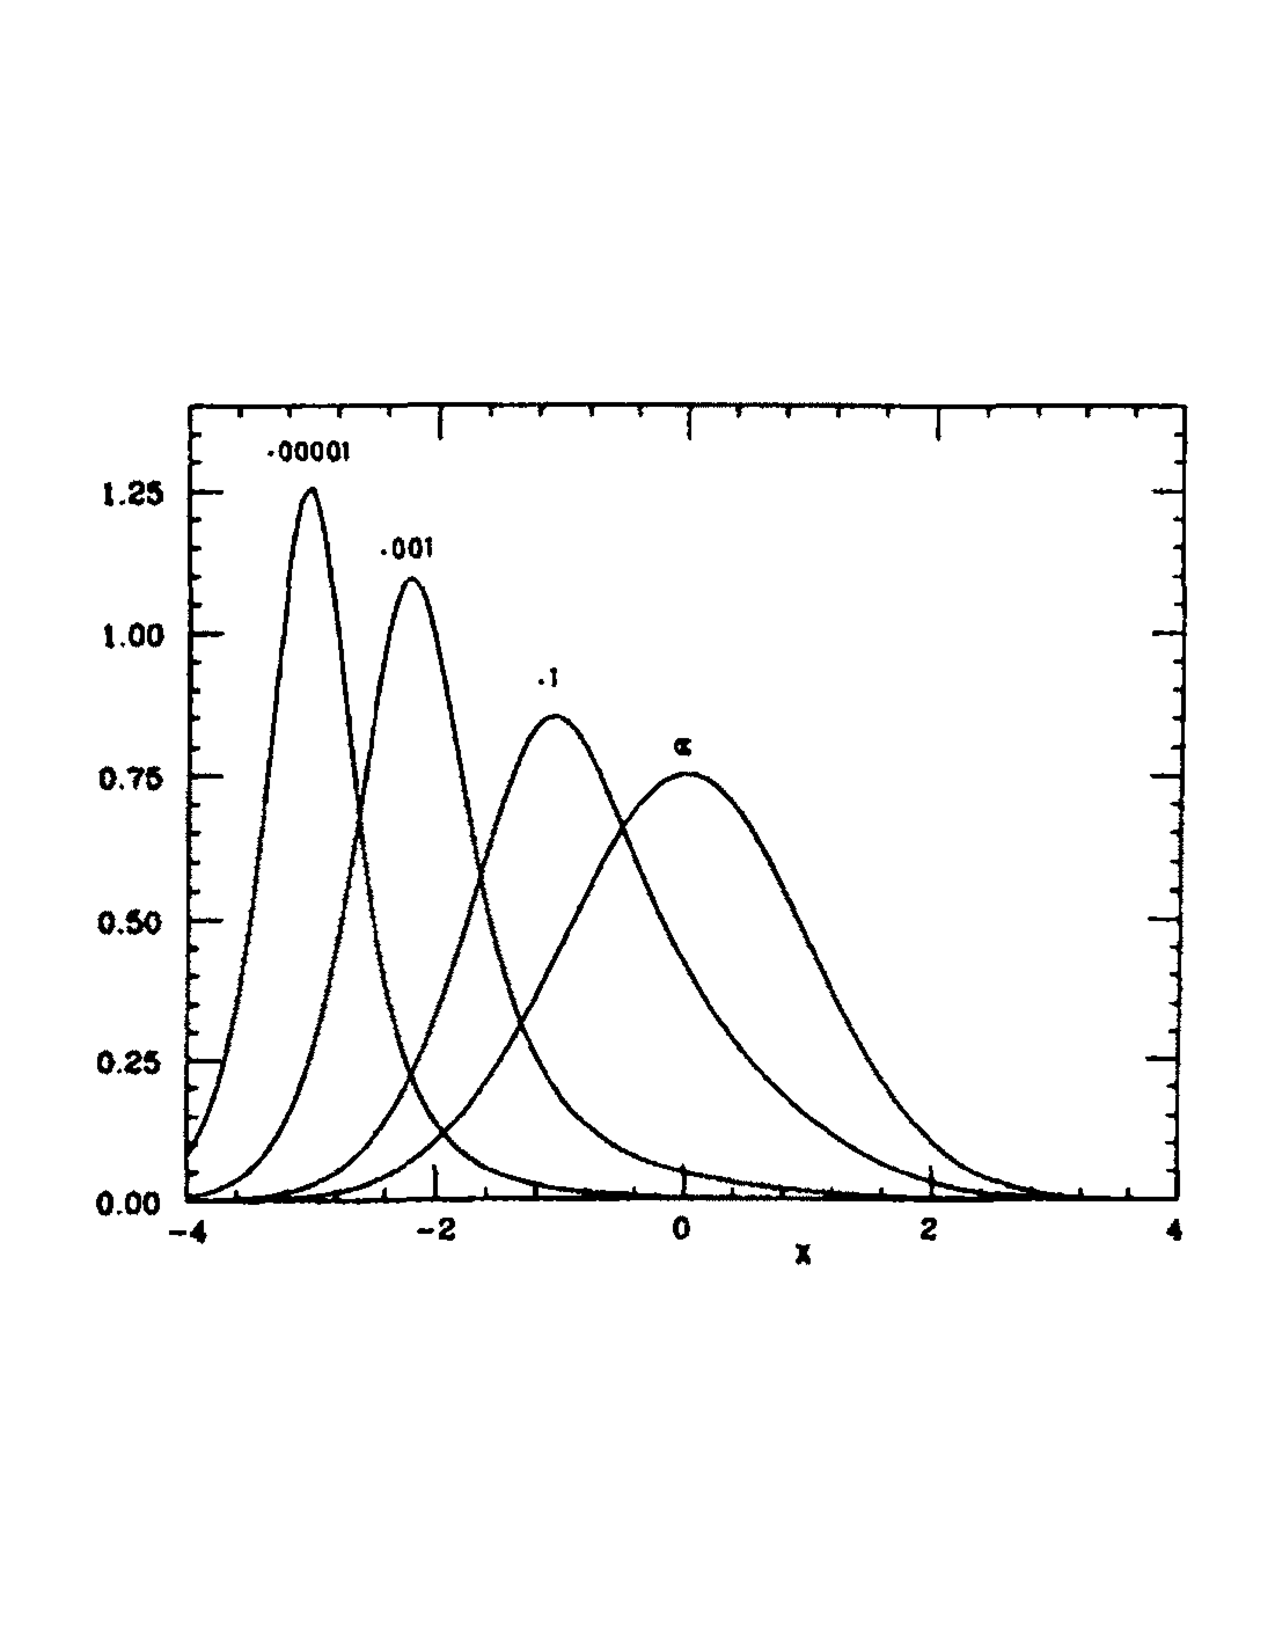
\includegraphics[height=8cm, keepaspectratio=1, trim=0cm 7cm 0cm 7cm]{pics/slika4}
	\caption{Graf prikazuje osnovne valovne funkcije k grafu iz slike~\ref{sl2}.}
	\label{sl3}
\end{figure}

Sedaj smo dobili dru\v zine potencialov, ki vrnejo vsa stanja ista, razen osnovnega, ki je odvisen od parametra $\lambda_1$.
Vendar gremo lahko korak dlje in isto naredimo za $V^{(2)}$, ki ga spremenimo v $\tilde{V}^{(2)}(x; \lambda_2)$, kar se potem
pomeni $V^{(1)} \to \tilde{V}^{(1)} (x; \lambda_1, \lambda_2)$. To lahko posplo\v simo na vsa vezana stanja in dobimo $\tilde{V}
^{(1)}(x; \underline{\lambda})$.

Taka dru\v zina potencialov, $\tilde{V}^{(1)}(x;\underline{\lambda})$, je popolnoma izospektralna, momente pa lahko nastavljamo
poljubno prek $\underline{\lambda}$.



%conclusion
\section{Conclusion}

Now you may ask yourself: how will the Higgs discovery affect me? How will this reflect on our daily lives? If the so
called ``God particle'' will be excluded, will this mean the end of the world? Well, regardless of the outcome, nothing
will change. In the best case scenario, some Nobel prizes will be awarded to the top brass and that's it. There is no bigger
mystery behind it apart from that the media created. These experiments serve only to round up the Standard Model and
the electroweak theory. Even if in the Higgs boson will be excluded, many technological breakthroughs had to be made
in other engineering sciences for the construction of such complex experiments so regardless of the outcome, we are gaining
something.

The Higgs boson mass has been narrowed down experimentally to 115 < $M_H$ < 127 (CMS) < 131 (ATLAS) GeV, with $\approx 4.7$ fb$^{-1}$
of data (integrated luminosity). After this year LHC will shut down for a longer period and resume in two years, hopefully
with it's design $\sqrt{s}$ and luminosity (this year the collisions are at $\sqrt{s} = 8$ TeV). During this shutdown, there
is enough data waiting to be analyzed.


\bibliographystyle{phjcp}
\bibliography{bib/bib1,bib/bib2,bib/bib3,bib/bib4,bib/bib5,bib/bib6,bib/bib7,bib/bib8,bib/bib9,bib/bib10,bib/bib11,bib/bib12,bib/bib13}

\end{document}
